\documentclass{beamer}\usepackage[]{graphicx}\usepackage[]{color}
%% maxwidth is the original width if it is less than linewidth
%% otherwise use linewidth (to make sure the graphics do not exceed the margin)
\makeatletter
\def\maxwidth{ %
  \ifdim\Gin@nat@width>\linewidth
    \linewidth
  \else
    \Gin@nat@width
  \fi
}
\makeatother

\definecolor{fgcolor}{rgb}{0.345, 0.345, 0.345}
\newcommand{\hlnum}[1]{\textcolor[rgb]{0.686,0.059,0.569}{#1}}%
\newcommand{\hlstr}[1]{\textcolor[rgb]{0.192,0.494,0.8}{#1}}%
\newcommand{\hlcom}[1]{\textcolor[rgb]{0.678,0.584,0.686}{\textit{#1}}}%
\newcommand{\hlopt}[1]{\textcolor[rgb]{0,0,0}{#1}}%
\newcommand{\hlstd}[1]{\textcolor[rgb]{0.345,0.345,0.345}{#1}}%
\newcommand{\hlkwa}[1]{\textcolor[rgb]{0.161,0.373,0.58}{\textbf{#1}}}%
\newcommand{\hlkwb}[1]{\textcolor[rgb]{0.69,0.353,0.396}{#1}}%
\newcommand{\hlkwc}[1]{\textcolor[rgb]{0.333,0.667,0.333}{#1}}%
\newcommand{\hlkwd}[1]{\textcolor[rgb]{0.737,0.353,0.396}{\textbf{#1}}}%

\usepackage{framed}
\makeatletter
\newenvironment{kframe}{%
 \def\at@end@of@kframe{}%
 \ifinner\ifhmode%
  \def\at@end@of@kframe{\end{minipage}}%
  \begin{minipage}{\columnwidth}%
 \fi\fi%
 \def\FrameCommand##1{\hskip\@totalleftmargin \hskip-\fboxsep
 \colorbox{shadecolor}{##1}\hskip-\fboxsep
     % There is no \\@totalrightmargin, so:
     \hskip-\linewidth \hskip-\@totalleftmargin \hskip\columnwidth}%
 \MakeFramed {\advance\hsize-\width
   \@totalleftmargin\z@ \linewidth\hsize
   \@setminipage}}%
 {\par\unskip\endMakeFramed%
 \at@end@of@kframe}
\makeatother

\definecolor{shadecolor}{rgb}{.97, .97, .97}
\definecolor{messagecolor}{rgb}{0, 0, 0}
\definecolor{warningcolor}{rgb}{1, 0, 1}
\definecolor{errorcolor}{rgb}{1, 0, 0}
\newenvironment{knitrout}{}{} % an empty environment to be redefined in TeX

\usepackage{alltt}
\usetheme[compress]{Singapore}
\useoutertheme{miniframes}

% \documentclass{beamer}
%\usetheme{Warsaw}

% Pour les documents en francais...
	\usepackage[latin1]{inputenc}
	\usepackage[french]{babel}
	\usepackage[french]{varioref}

% Math�matiques
	\usepackage{amsmath}

% Caracteres speciaux suppl�mentaires
	\usepackage{latexsym,amsfonts}

% A documenter
	\usepackage{moreverb}

% Macros pour les paquets
	\usepackage{array}  			% N�cessaires pour les tableaux de la macro Excel.

% Outil suppl�mentaire pour les tableaux
	\usepackage{multirow}
	\usepackage{booktabs}
	\usepackage{xcolor} % alternating row colors in table, incompatible avec certains modules
	\usepackage{longtable}
	\usepackage{colortbl}

% Pour ins�rer des graphiques
	\usepackage{graphicx} 			% Graphique simples
	\usepackage{subfigure}			% Graphiques multiples

% Pour ins�rer des couleurs
	\usepackage{color}

% Rotation des objets et des pages
%	\usepackage{rotating}
%	\usepackage{lscape}

% Pour insrer du code source, LaTeX ou SAS par exemple.
	\usepackage{verbatim}
        \usepackage{moreverb}
	\usepackage{listings}
	\usepackage{fancyvrb}

%	\lstset{language=SAS,numbers=left}		% Par dfaut le listing est en SAS

% Pour ins�rer des hyperliens
  \usepackage{hyperref}

% American Psychological Association (for bibliographic references).
	\usepackage{apacite}

% Pour l'utilisation des macros
	\usepackage{xspace}

% Pour l'utilisation de notes en fin de document.
%	\usepackage{endnotes}

% Array
%	\usepackage{multirow}
%	\usepackage{booktabs}

% Rotation
%	\usepackage{rotating}

% En t�tes et pieds de pages
%	\usepackage{fancyhdr}
%	\usepackage{lastpage}


% Page layout

% By LaTeX commands
%\setlength{\oddsidemargin}{0cm}
%\setlength{\textwidth}{16cm}
%\setlength{\textheight}{24cm}
%\setlength{\topmargin}{-1cm}
%\setlength{\marginparsep}{0.2cm}

% fancyheader parameters
%\pagestyle{fancy}

%\fancyfoot[L]{{\small Formation \LaTeX, DEPP}}
%\fancyfoot[c]{}
%\fancyfoot[R]{{\small \thepage/\pageref{LastPage}}}

%\fancyhead[L]{}
%\fancyhead[c]{}
%\fancyhead[R]{}


% Pour ins�rer des dessins de Linux
\newcommand{\LinuxA}{\includegraphics[height=0.5cm]{Graphiques/linux.png}}
\newcommand{\LinuxB}{\includegraphics[height=0.5cm]{Graphiques/linux.png}\xspace}

% Macro pour les petits dessins pour les diff�rents OS.
\newcommand{\Windows}{\emph{Windows}\xspace}
\newcommand{\Mac}{\emph{Mac OS X}\xspace}
\newcommand{\Linux}{\emph{Linux}\xspace}
\newcommand{\MikTeX}{MiK\tex\xspace}

\newcommand{\df}{\emph{data.frame}\xspace}
\newcommand{\dfs}{\emph{data.frames}\xspace}
\newcommand{\liste}{\emph{list}\xspace}
\newcommand{\listes}{\emph{lists}\xspace}

\newcommand{\factor}{\emph{factor}\xspace}
\newcommand{\character}{\emph{character}\xspace}
\newcommand{\logical}{\emph{logical}\xspace}

\newcommand{\cad}{c'est-�-dire\xspace}

\newcommand{\hreff}[2]{\underline{\href{#1}{#2}\xspace}}


% Titre
\title{Introduction � R}
\author{Pascal Bessonneau}
%\institute{DEPP}
\date{06/2015}
\subtitle{Clustering}

\begin{knitrout}
\definecolor{shadecolor}{rgb}{0.969, 0.969, 0.969}\color{fgcolor}\begin{kframe}


{\ttfamily\noindent\itshape\color{messagecolor}{\#\# Loading required package: FactoMineR}}\end{kframe}
\end{knitrout}

\IfFileExists{upquote.sty}{\usepackage{upquote}}{}
\begin{document}

\begin{frame}
	\maketitle
\end{frame}

\begin{frame}
	\tableofcontents
\end{frame}

% Begin document %%%%%%%%%%%%%%%%%%%%%%%%%%%%%%%%%%%%%%%%%%%%%%%%%%%%%%%%%%%%%%%%%%%%%%%%%%%%%%%%%%

\section{Cluster}

\begin{frame}[containsverbatim]
	\frametitle{Le principe}

  Le principe est � partir des variables de calculer la distance entre individus
  et de grouper les individus les plus proches.
  
\end{frame}

\begin{frame}[containsverbatim]
	\frametitle{Temp�rature}

Nous utilisons toujours les donn�es sur la temp�rature.

\begin{knitrout}\footnotesize
\definecolor{shadecolor}{rgb}{0.969, 0.969, 0.969}\color{fgcolor}\begin{kframe}
\begin{alltt}
\hlstd{temp} \hlkwb{<-} \hlkwd{read.csv2}\hlstd{(}\hlstr{"data/temp.csv"}\hlstd{)}
\hlkwd{colnames}\hlstd{(temp)}
\end{alltt}
\begin{verbatim}
##  [1] "Ville"     "Janvier"   "Fevrier"  
##  [4] "Mars"      "Avril"     "Mai"      
##  [7] "Juin"      "Juillet"   "Aout"     
## [10] "Septembre" "Octobre"   "Novembre" 
## [13] "Decembre"  "lati"      "long"
\end{verbatim}
\end{kframe}
\end{knitrout}

\end{frame}

\begin{frame}[containsverbatim]
	\frametitle{Pr�paration des donn�es}

Dans ce cas il faut centrer et r�duire les donn�es pour �viter les probl�mes
de diff�rence d'unit�s.

\begin{knitrout}\footnotesize
\definecolor{shadecolor}{rgb}{0.969, 0.969, 0.969}\color{fgcolor}\begin{kframe}
\begin{alltt}
\hlstd{numerics} \hlkwb{<-} \hlkwd{sapply}\hlstd{(temp,is.numeric)}
\hlkwa{for} \hlstd{(ii} \hlkwa{in} \hlkwd{which}\hlstd{(numerics))}
  \hlstd{temp[[ii]]} \hlkwb{<-} \hlkwd{scale}\hlstd{(temp[[ii]])}
\end{alltt}
\end{kframe}
\end{knitrout}

\end{frame}

\begin{frame}[containsverbatim]
  \frametitle{Peut-on r�sumer les informations ?}

\begin{knitrout}\footnotesize
\definecolor{shadecolor}{rgb}{0.969, 0.969, 0.969}\color{fgcolor}\begin{kframe}
\begin{alltt}
\hlstd{hcpc} \hlkwb{<-} \hlkwd{HCPC}\hlstd{(temp[,}\hlnum{1}\hlopt{:}\hlnum{12}\hlstd{],}\hlkwc{nb.clust} \hlstd{=} \hlnum{3}\hlstd{)}
\end{alltt}


{\ttfamily\noindent\bfseries\color{errorcolor}{\#\# Error in FUN(data[x, , drop = FALSE], ...): 'x' doit �tre num�rique}}\end{kframe}

{\centering 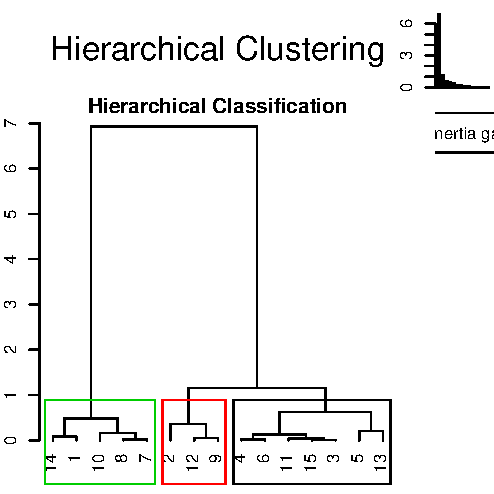
\includegraphics[width=\textwidth]{graphiques/beamer-unnamed-chunk-4-1} 

}



\end{knitrout}

\end{frame}


\begin{frame}[containsverbatim]
	\frametitle{R�sultats}

Nous pouvons voir � la longueur des branches de l'arbre quelles sont les villes
les plus proches les unes des autres. 

Apr�s l'algorithme nous propose une coupure optimale � 3 groupes.

\end{frame}

\begin{frame}[containsverbatim]
  \frametitle{R�sultats}

Nous avons 1 groupe qui r�unit les villes les plus au sud, un cluster
qui r�unit les villes de Bretagne au climat peu continental avec 
peu de variations entre les temp�ratures extr�mes et les villes au climat 
plus continental et situ� au nord de la Loire.
  
\end{frame}



\begin{frame}[containsverbatim]
  \frametitle{R�sultats}
  
  Le clustering fait partie des m�thodes de \emph{Machine Learning} qui 
  permettent d'analyser les comportements consomnateurs et du profilage
  des individus sur internet.

\end{frame}


  

\end{document}

